%%%%%%%%%%%%%%%%%%%%%%%%%%%%%%%%%%%%%%%%%
% Thin Sectioned Essay
% LaTeX Template
% Version 1.0 (3/8/13)
%
% This template has been downloaded from:
% http://www.LaTeXTemplates.com
%
% Original Author:
% Nicolas Diaz (nsdiaz@uc.cl) with extensive modifications by:
% Vel (vel@latextemplates.com)
%
% License:
% CC BY-NC-SA 3.0 (http://creativecommons.org/licenses/by-nc-sa/3.0/)
%
%%%%%%%%%%%%%%%%%%%%%%%%%%%%%%%%%%%%%%%%%

%----------------------------------------------------------------------------------------
%	PACKAGES AND OTHER DOCUMENT CONFIGURATIONS
%----------------------------------------------------------------------------------------

\documentclass[a4paper, 11pt]{article} % Font size (can be 10pt, 11pt or 12pt) and paper size (remove a4paper for US letter paper)

\usepackage[protrusion=true,expansion=true]{microtype} % Better typography
\usepackage{graphicx} % Required for including pictures
\usepackage{wrapfig} % Allows in-line images
\usepackage[paper=a4paper,left=25mm,right=25mm,top=25mm,bottom=25mm]{geometry}

\renewcommand{\familydefault}{\sfdefault}
\usepackage{helvet} % Use the Palatino font
\usepackage[T1]{fontenc} % Required for accented characters
\usepackage[format=plain,footnotesize,labelfont=bf,justification=justified,singlelinecheck=false]{caption}


\linespread{1.05} % Change line spacing here, Palatino benefits from a slight increase by default



\makeatletter
\renewcommand\@biblabel[1]{\textbf{#1.}} % Change the square brackets for each bibliography item from '[1]' to '1.'
\renewcommand{\@listI}{\itemsep=0pt} % Reduce the space between items in the itemize and enumerate environments and the bibliography

\renewcommand{\maketitle}{ % Customize the title - do not edit title and author name here, see the TITLE block below
\begin{flushright} % Right align
{\LARGE\@title} % Increase the font size of the title

\vspace{20pt} % Some vertical space between the title and author name

{\large\@author} % Author name
\\\@date % Date

\vspace{10pt} % Some vertical space between the author block and abstract
\end{flushright}
}

%----------------------------------------------------------------------------------------
%	TITLE
%----------------------------------------------------------------------------------------

\title{\textbf{Co-regulation of NER repair factor expression}\\ % Title
Third TAC-meeting} % Subtitle

\author{\textit{Tim Heinemann} % Author
\\{\textit{Theoretical Systems Biology (AG H�fer)}}} % Institution

\date{\textit{\today}} % Date

%----------------------------------------------------------------------------------------

\begin{document}

\maketitle % Print the title section

%----------------------------------------------------------------------------------------
%	ABSTRACT AND KEYWORDS
%----------------------------------------------------------------------------------------

%\renewcommand{\abstractname}{Summary} % Uncomment to change the name of the abstract to something else

%----------------------------------------------------------------------------------------
%	ESSAY BODY
%----------------------------------------------------------------------------------------

\section*{Introduction}

The recently published model-aided analysis of the DNA repair process revealed a link between the emergent phenomenon of rapidly exchanging and transiently interacting NER (nuclear excision repair) components with the experimentally observed slow first-order kinetics of repair \cite{Verbruggen2014}. An important functional consequence of this kinetic design is that the control of the repair rate is shared by all repair factors. This manifests in the mathematical prediction of uniformly distributed response coefficients, which quantify the relative change of the repair rate in answer to changes in the nuclear repair protein concentration. Exploiting the natural variability in NER factor expression we experimentally corroborated the moderate control of the repair components on the repair rate. However, these findings were made under the assumption of a functional independence of the individual NER components. Upstream  effects regulating the repair rate due to NER factor co-expression were so far not considered.  \\
To test this assumption, we experimentally investigate the potential cross-correlation between five repair factors (XPC, TFIIH, XPA, XPF and RPA). Surprisingly, we find that the nuclear expression of these pairwise measured repair factors is indeed strongly positively correlated, whereas there is no correlation with the repair-independent cell cycle marker Ki67. This result suggests an additional control mechanism orchestrating NER factor expression on the transcriptional or translational level. 


\section*{Nuclear expression of NER factors is strongly correlated}

Using fluorescence microscopy for the quantitative analysis of the NER process proved to result in accurate measurements of the nuclear repair factor expression and their UV-induced repair dynamics. This applies for the detection of stably transfected fluorescently tagged repair proteins as well as for an immunocytochemistry approach with an indirect antibody-labeling of the measured NER factors. The latter has the additional advantage that it allows for a flexible combinatorial tagging of multiple antigens simultaneously.\\  
\noindent We used an indirect antibody-labeling protocol for seven single cell double stainings (XPC-XPC; XPC-TFIIH; XPC-XPA; XPC-XPF; XPC-RPA; TFIIH-XPF; XPA-XPF; XPA-RPA) of human diploid female fibroblasts and subsequently performed a protein expression cross-correlation analysis of this single-cell data. The pairwise co-expression was quantified by 3-dimensional imaging with a confocal microscope. To test whether the antibody co-staining experiment is suitable for the cross-correlation analysis we measured XPC expression with a directly labeled antibody together with an indirect immuno-staining and correlated both signals (cf.\ Figure \ref{fig:Mic_nucCorrel}A). The measurement error was determined using a principal components analysis. ... Hence, this approach is sufficiently accurate to exploit the natural variability in protein expression for the cross-correlation analysis. 


\begin{figure}[htbp]
	\begin{center}
		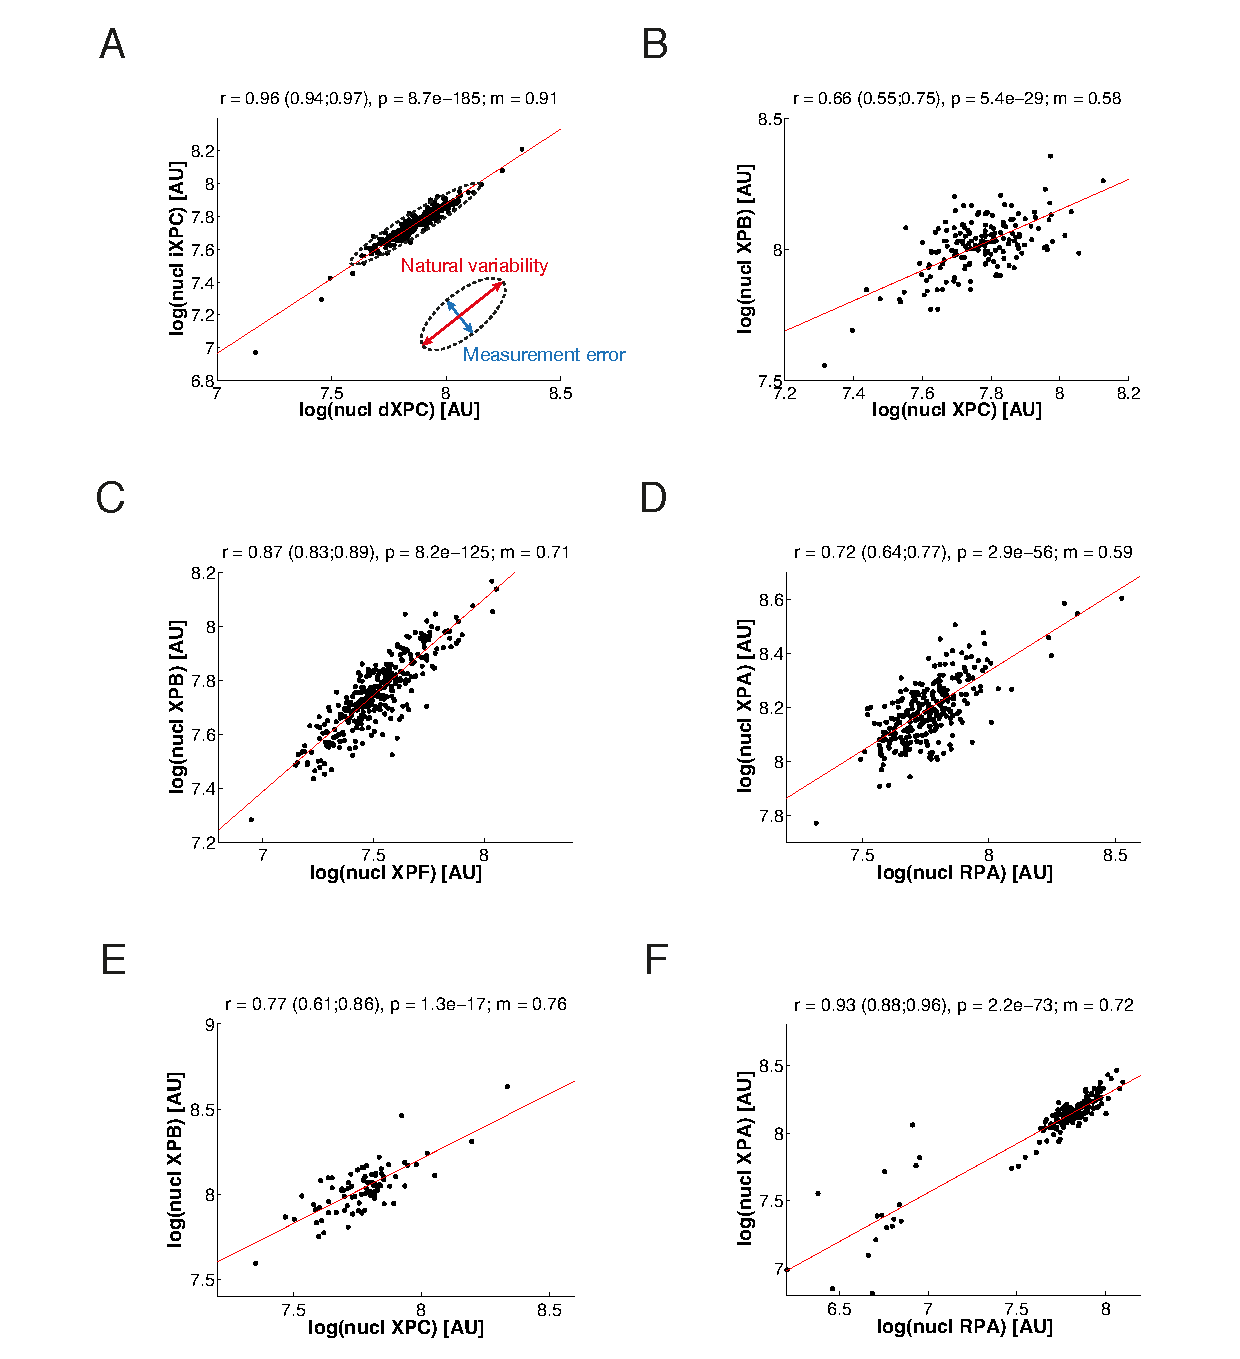
\includegraphics[width=1\textwidth]{Abbildungen/figureTAC_2.pdf}
		\caption{\textbf{NER factor cross-correlation is repair independent.} A) Scatter plot of indirectly antibody-stained XPC against a directly labeled antibody recognizing XPC (n=336) as determined by quantitative (immuno) fluorescence microscopy. B-D) Pairwise correlations of indirectly antibody-labeled XPB against XPC (n=220, B), XPB against XPF (n=410, C) and XPA against RPA (n=350, D) in locally damaged cells. Expression values represent fluorescence intensities originating from the nucleus including the damaged region (signal quantification was performed analogous to \cite{Luijsterburg2010}). E-F) Scatter plots of the nuclear expression of XPB vs. XPC (n=85) and XPA vs. RPA (n=170) in undamaged cells. A-F) Red lines represent linear regression with correlation coefficient r, p-value and slope m. 95\% confidence bounds of all correlation coeffiecients r were estimated by non-parametric bootstrap and are given in brackets. }
		\label{fig:Mic_nucCorrel}
	\end{center}
\end{figure}


\noindent As it turns out, all pairwise correlations of the measured co-staining experiments are strongly positively correlated with correlation coefficients between 0.74 and 0.88 (cf.\ Figure \ref{fig:Mic_nucCorrel}B-D (only selected pairs)). Notably, the result is irrespective of whether the acquired fluorescence signal is taken from the whole nucleus including the locally damaged area or only from the undamaged chromatin region (cf.\ Figure \ref{fig:Mic_nucCorrel}B-D and \ref{fig:Mic_nucCorrel}E-F). This suggests that the correlation of nuclear NER factors is independent of the ongoing repair. As a consequence, we suspect that the regulatory mechanism determining the protein concentrations lies on a preceding level such as transcription or translation.\\  
To further pursue this question we repeated the experiment by flow cytometry, this time, investigating the NER-factor expression in human brain pericytes. We established a double-staining protocol for XPA and RPA and observed that also in this cell type the two repair factors strongly correlate (cf.\ Figure \ref{fig:FACS_nucCorrel}A and B).     

\begin{figure}[htbp]
	\begin{center}
		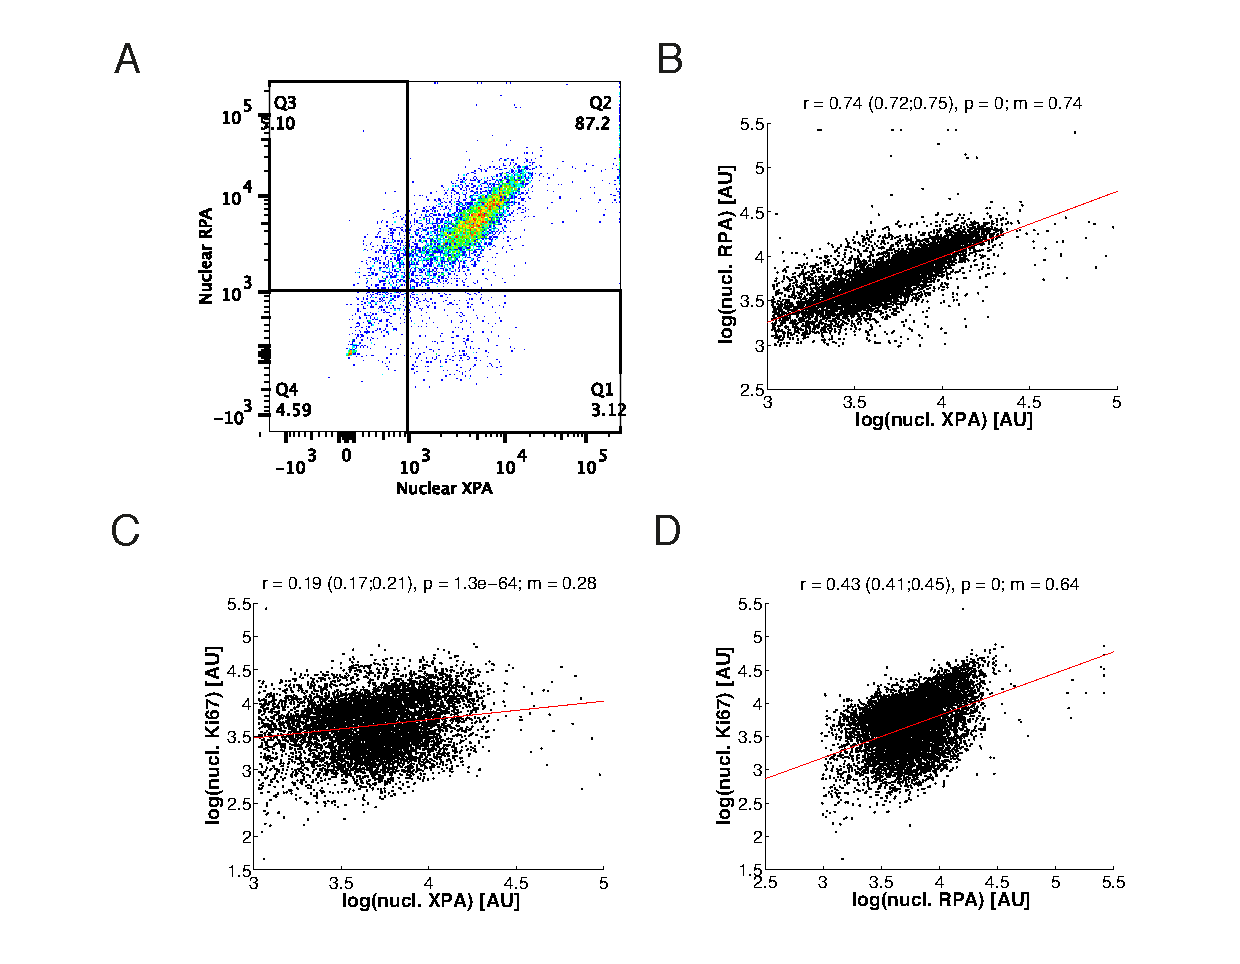
\includegraphics[width=1\textwidth]{Abbildungen/figureTAC_3.pdf}
		\caption{\textbf{Correlated expression of RPA and XPA in human brain pericytes} A) Selection of XPA and RPA positive human brain pericytes (Q2) as determined by flow cytometry (n=8084). B-D) Nuclear expression of indirectly antibody-labeled RPA against XPA (B), Ki67 against XPA (C) and Ki67 against RPA (D). B-D) Red lines represent linear regression with correlation coefficient r, p-value and slope m. 95\% confidence bounds of all correlation coeffiecients r were estimated by non-parametric bootstrap and are given in brackets.}
		\label{fig:FACS_nucCorrel}
	\end{center}
\end{figure}

\noindent Quantitatively, the correlation coefficients of the double-staining signals in both cell types have the same order of magnitude. In particular, each value falls into the confidence interval of the other (cf.\ Figure \ref{fig:FACS_nucCorrel}B and Figure \ref{fig:Mic_nucCorrel}D). To test, whether this correlation is specific for proteins involved in DNA repair we measured the expression of the proliferation marker Ki67. Surprisingly, although the correlation between both repair factors and Ki67 is visibly reduced (XPA vs. Ki67 = 0.19 and RPA vs. Ki67 = 0.43 against XPA-RPA = 0.73) it is still significantly positive (cf.\ Figure \ref{fig:FACS_nucCorrel}C and D). 


\section*{Cell cycle independent cross-correlation of NER factor expression}
As Ki67 increases during cell cycle we asked, to what extend the observed protein correlation of Ki67 and the NER factors is cell-cycle dependent? To answer this question, we stained the cell's DNA using FxCycle violet and gated them according to their DNA content (cf.\ Figure \ref{fig:CellCycle_nucCorrel}A). Two distinct peaks denote the portion of cells traversing the G1 or the synthesis and G2 phase, respectively. By sorting the protein expression values in accordance with their cell cycle phase we identified for each protein combination two contiguous regions revealing a general trend of increased protein expression during the S1 and G2 phase in comparison to the G1 phase (cf.\ Figure \ref{fig:CellCycle_nucCorrel}B-D).          

\begin{figure}[htbp]
	\begin{center}
		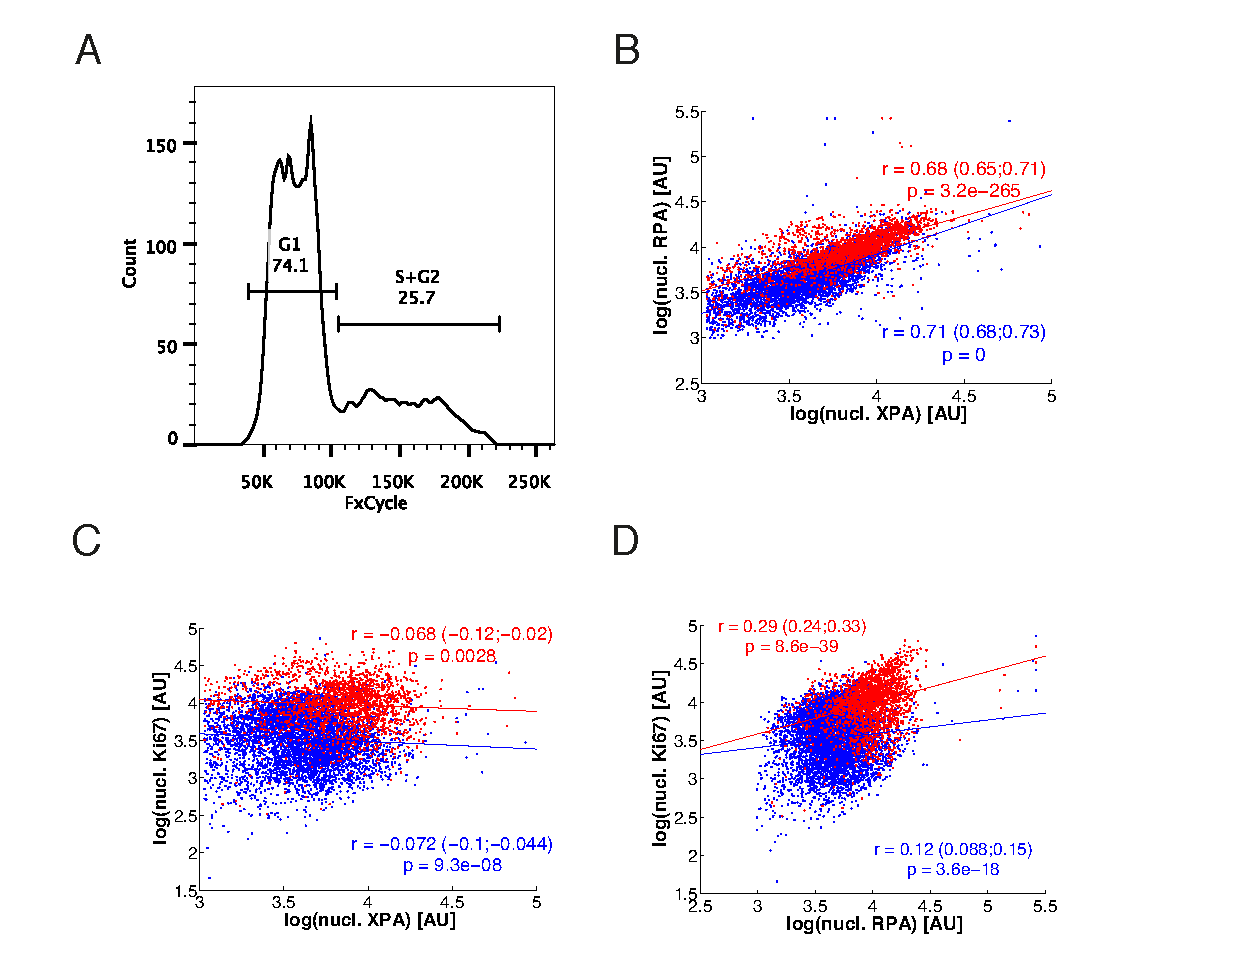
\includegraphics[width=1\textwidth]{Abbildungen/figureTAC_4.pdf}
		\caption{\textbf{NER factor cross-correlation is robust against cell cycle progression.} A) Distribution of fluorescently labeled DNA proportional to the DNA content. Horizontal bars indicate the fractions of cells assigned to G1 (left peak, n=5469) and S+G2 (right peak, n=1945).  B-D) Individual regression analysis of the nuclear expression values sorted according to the corresponding cell-cycle phase (G1 - blue; S+G2 - red) for RPA vs. XPA (B), Ki67 vs. XPA (C) and Ki67 vs. RPA (D). B-D) Red and blue lines represent linear regression with correlation coefficient r and p-value. 95\% confidence bounds of all correlation coeffiecients r were estimated by non-parametric bootstrap and are given in brackets.}
		\label{fig:CellCycle_nucCorrel}
	\end{center}
\end{figure}

\noindent Remarkably, whereas the correlation coefficients between XPA and RPA remain constant for both regimes (G1: 0.71, S+G2: 0.68, all: 0.74) the correlation between XPA and Ki67 disappear (G1: -0.072, S+G2: -0.068). Between RPA and Ki67 there is close to no correlation in the G1 phase but a significant small positive correlation in the S and G2 phase (G1: 0.12, S+G2: 0.29). These results strengthen the conclusions derived from the cross-correlation analysis in fibroblasts that NER factor expression is functionally co-regulated. In particular, the missing correlation between the nuclear factors and the cell cycle marker after taking the cell-cycle into account suggests that the measured correlation is specific to NER proteins. 

\section*{Conclusion}

To determine potential mutual dependencies in NER factor expression we performed two independent cross-correlation experiments, firstly based on microscopy of human fibroblast and secondly using flow cytometry in human brain pericytes. For both approaches we found conclusive evidence for a positive pairwise correlation of the nuclear repair factor concentration. We could show that the correlation is independent of the repair process and the cell cycle phase despite the general elevation of the protein expression levels in the S and G2 phase compared to G1. This result indicates a so far unknown regulatory step organizing the repair factor co-expression, which has to be considered when determining the control on the rate of repair.



%----------------------------------------------------------------------------------------
%	BIBLIOGRAPHY
%----------------------------------------------------------------------------------------

\footnotesize\bibliographystyle{naturemagC}
\bibliography{NER_Bibliography}

%----------------------------------------------------------------------------------------

\end{document}